\documentclass[12pt,]{article}
\usepackage{beamerarticle}
\usepackage[utf8]{inputenc}
\usepackage{hyperref}
\hypersetup{%
  colorlinks=true,% hyperlinks will be coloured
  citecolor={blue!50!black},
  urlcolor={blue!80!black},
  linkcolor=blue,% hyperlink text will be green
  linkbordercolor=blue,% hyperlink border will be red
}

% Math
\usepackage{amssymb,amsmath,amsthm} 
\theoremstyle{plain} % other formats: definition, plain, remark
\newtheorem{proposition}{Proposition}
\newtheorem{define}{Definition}

% Fontfamily
\usepackage{palatino}%\usepackage{lmodern, times}

% Page settings
\usepackage[letterpaper, margin=1in]{geometry}
\usepackage{setspace}                           
\onehalfspacing %\doublespacing  % \singlespacing 

% Appendix
\usepackage{appendix}

% Line numbers
%\usepackage{lineno}
%\linenumbers


% Tables
\usepackage{dcolumn}
\usepackage{array,booktabs,longtable,rotating}
\newenvironment{tablenotes}[1][]{
  \begin{minipage}{\textwidth}\emph{Notes:}{\footnotesize #1}
}{\end{minipage}}
\makeatletter
\def\fps@table{htbp}
\makeatother

% Graphics
\usepackage{graphicx,grffile}
\makeatletter
\def\maxwidth{\ifdim\Gin@nat@width>\linewidth\linewidth\else\Gin@nat@width\fi}
\def\maxheight{\ifdim\Gin@nat@height>\textheight\textheight\else\Gin@nat@height\fi}
\makeatother
% Scale images if necessary, so that they will not overflow the page
% margins by default, and it is still possible to overwrite the defaults
% using explicit options in \includegraphics[width, height, ...]{}
\setkeys{Gin}{width=\maxwidth,height=\maxheight,keepaspectratio}
% set default figure placement to htbp
\makeatletter
\def\fps@figure{htbp}
\makeatother

\usepackage{natbib}% plainnat
\bibliographystyle{aer}


\setlength{\emergencystretch}{3em}  % prevent overfull lines
\providecommand{\tightlist}{%
  \setlength{\itemsep}{0pt}\setlength{\parskip}{0pt}}


\usepackage{framed}
\colorlet{shadecolor}{orange!15}


% Thresholds, limits, bounds, etc.
\newcommand\deadline{\bar{t}}
\newcommand\target{\underline{y}}

% Competitions
\newcommand\race{\text{race}}
\newcommand\tournament{\text{tour}}

% Cost functions
\newcommand\ctime{c_{t}}
\newcommand\cscore{c_{y}}
\newcommand\cability{c_{a}}
\newcommand\costs{\cability(a_i)\cscore(y_i)\ctime(t_i)}

% Distribution of types
\newcommand\ability{a_i}
\newcommand\marginaltype{\underline{a}}
\newcommand\mtype{\underline{a}}
\newcommand\lotype{\underline{a}}
\newcommand\hitype{\bar{a}}



% Derivatives
\newcommand\dystar{\frac{\partial y^*(x,\target)}{\partial\target}dF_{N:N}(x)}

\title{Races or Tournaments? {[}PRELIMINARY AND INCOMPLETE{]}\thanks{Blasco: Harvard Institute for Quantitative Social Science, Harvard
University, 1737 Cambridge Street, Cambridge, MA 02138 (email:
\href{mailto:ablasco@fas.harvard.edu}{\nolinkurl{ablasco@fas.harvard.edu}}).}}
\author{Andrea Blasco \and Kevin J. Boudreau \and Karim R. Lakhani \and Michael Menietti}
\date{Last updated: 23 February, 2017}

\begin{document}
\maketitle
\begin{abstract}
Contests are often used as incentive schemes to foster innovation. The
typical goal of contest designers is to maximize quality while
minimizing the time it takes to achieve the innovation. This situation
leads to a difficult choice of design made under considerable
uncertainty. In this study, we investigate one key aspect of this
decision that is the way participants compete. Two extreme forms of
competition are considered: the race, where the first to achieve the
innovation wins, and the tournament, where the timing is not important.
We develop a model to characterize under what conditions contest
designers should go for one or the other approach. Then, we report the
results of a field experiment conducted to compare the outcomes of three
alternative competitive situations motivated by theory: the race, the
tournament, and the tournament with a quality requirement. We find that
outcomes in a race are of comparable quality, but are supplied faster.
Based on our model, we also show what would be optimal to do under
several simulated counterfactual situations.

\smallskip\noindent 
JEL Classification: xxx; xxx; xxx.

\smallskip\noindent 
Keywords: xxxx; xxxx xxxx.
\end{abstract}


% Todo notes
%\usepackage[textsize=tiny]{todonotes}
%\newcommand\redmarginpar[1]{\marginpar{\footnotesize{\textcolor{red}{#1}}}}
%\listoftodos[Notes]
\clearpage
\tableofcontents
\setcounter{tocdepth}{2}
\clearpage

\section{Introduction}\label{introduction}

Organizations often use contests as incentive schemes to foster
innovation. In an innovation contest, participants compete for prizes by
investing time and energy in an innovation project. The typical aim of
the contest designer is to maximize quality while minimizing the time to
complete the innovation. Balancing between these two desirable but
incompatible features it is often difficult. The lack of knowledge about
individual costs and technical feasibility of the innovation may force
contest designers to make their choices under considerable uncertainty.
A growing literature on contest design offers insights on how to make
better resolutions. However, while researchers have examined various
aspects of managing this trade-off, the optimal design is still largely
unknown.

Here, we investigate one key aspect of contest design concerning the way
participants compete. There are two extreme forms of competition that we
consider. One is the \emph{race} where the first to finish an innovation
project wins. The second is the \emph{tournament} where the best
finished project wins. To fix ideas, imagine a government designing an
innovation contest to find a solution to a threat to the public health,
such as the UK government on the problem of antibiotic
resistance.\footnote{This example is taken\ldots{}} To minimize the
risks that the threat will materialize before a solution is found, one
choice is a tournament competition with a tight deadline for
participants to provide their solutions. Alternatively, the government
can use a race competition awarding a prize to the first participant
that achieves, or goes beyond, a minimum effectiveness threshold. Fixed
the prize, both approaches have specific advantages and limitations. If
the duration of the competition is too low, a tournament may give
insufficient incentives resulting in inadequate solutions. In a race
competition, instead, timing is not an issue but participants have no
incentives to exceed the minimum threshold.

In the present study, we shed light on the conditions under which
contest designers should choose between a race and a tournament
competition. We proceed in two ways. First, we develop a contest model
that encompasses both the race and the tournament in a single framework.
Exploring the duality of the model, we compare equilibrium behaviors
under both regimes and characterize the optimal choice (i.e., the setup
that maximizes the utility of the contest designer). Then, we design and
execute an experiment to test the implications of the theory in the
field, providing policy recommendations.

Regarding to the modeling, we adapt the contest model introduced by
\citet{moldovanu2001optimal}. Contests have an all-pay structure by
which participants pay an immediate cost for an uncertain future reward.
We generalize by allowing participants to choose the timing and quality
of the innovation at once. This decision is made under the uncertainty
of the costs of the rivals, which are privately observed by the agents.
The contest designer is modeled as an extra agent with preferences for
both time and quality. Following the analysis of the model model, we
show that the optimal design depends on the number of participants and
the concavity of their cost function.

The field experiment was conducted at the end of 2016. The context of
the experiment was an online programming competition. In a programming
competition, participants compete writing source code that solves a
given problem for winning a monetary prize. We worked together with
researchers from the United States National Health Institute (NIH) and
the Scripps Research Institute (SCRIPPS) to select a challenging problem
for the contest. The selected problem was based on an algorithm called
BANNER built by NIH \citep{leaman2008banner} that uses expert labeling
to annotate abstracts from a prominent life sciences and biomedical
search engine, PubMed, so disease characteristics can be more easily
identified. The goal of the programming competition was to improve upon
the current NIH's system by using a combination of expert and non-expert
labeling, as described by \citet{good2014microtask}. The competition was
hosted online on the platform Topcoder.com (about 1M registered users in
2016). Top submissions were awarded monetary prizes ranging between
\$100 to \$5000 for a total prize pool of more than \$40,000.

Our intervention consisted in sorting at random participants into
independent virtual rooms of 10 or 15 people. These virtual rooms were
then randomly assigned to one of three different competitive settings: a
race, a tournament, and a tournament with a reserve score, which is the
lowest acceptable score by the platform for a submission to be awarded a
prize.

We find that xxxxx {[}participation in the tournament is xxx compared to
the race the reserve.{]}

We also find that xxxx {[}submission are quicker in a race, whereas are
equally distributed at the end of the competition in the the tournament
and in the tournament with quality requirement.{]}

Another interesting finding is that xxxxx {[}No evidence trade-off
between a race and a tournament in terms of higher scores vs faster
submissions. We do find that scores are higher in the tournament but we
do not find a strong trade-off in the sense that race had comparable
good quality solutions than the tournament.{]}

\section{Literature}\label{literature}

This paper is related to the contest theory literature
\citet{dixit1987strategic} \citet{baye2003strategic},
\citet{parreiras2010contests}, \citet{moldovanu2001optimal},
\citet{moldovanu2006contest}, \citet{siegel2009all},
\citet{siegel2014contests}. It also relates to the literature on
innovation contests \citet{taylor1995digging}, \citet{che2003optimal}.
And the personnel economics approach to contests \citet{lazear1981rank},
\citet{green1983comparison}, \citet{mary1984economic}.

Empirically, \citet{dechenaux2014survey} provide a comprehensive summary
of the experimental literature on contests and tourments. Large body of
empirical works have focused on sports contests
\citet{szymanski2003economic}. More recently, inside firms (xxx) and
online contest (xxxx).

This paper is also related to the econometrics of auctions
\citet{paarsch1992deciding}, \citet{laffont1995econometrics},
\citet{donald1996identification} and more recently
\citet{athey2011comparing}, \citet{athey2002identification}, and
\citet{athey2007nonparametric}.

An extensive literature has discussed the reasons why contests are
sometimes preferred to other forms of incentives (e.g., individual
contracts). Typically, contests reduce monitoring costs {[}xxx{]},
incentivize production with common risks {[}xxx{]}, and deal with
indivisible rewards {[}xxxx{]}, among others. While there is not much
debate on why contests should be used, the issue of how to effectively
design and deploy a contest still attracts much research.

Several aspects of contest design have been investigated, including the
optimal prize structure {[}XXX, xxxx, xxxx{]}, number of competitors
{[}XXX, XXX{]}, and imposing restrictions to competition such as minimum
effort requirements {[}XXX, XXX{]}. Also, a great deal of theoretical
models of races and tournaments have been developed and applied to a
wide range of economic situations including patent races {[}xxx{]}, arms
races {[}xxx{]}, sports {[}xxx{]}, the mechanism of promotions inside
firms {[}xxxx{]}, sales tournaments {[}xxxx{]}, etc.

\citet{harris1987racing}, \citet{grossman1987dynamic} investigate the
dynamics issues patent races where the interest is how firms compete for
a patent. \citet{bimpikis2014designing} looks at the problem of how to
design an information structure that is optimal when the contest is a
race and innovation is uncertain (encouragement and competition effect).
In the laboratory, \citet{zizzo2002racing} finds poor support to
predictions of dynamic xxxx. In general we do not know much about the
dynamic aspect of contests.

The duality. As pointed out by \citet{baye2003strategic}, many of these
models of tournament and race competitions are specific cases of a more
general ``contest games.'' And sometimes it is possible to design one or
the other in a way to exploit a ``duality.'' In other words, in theory,
a competition can be designed as a tournament to do xxx or as a race to
do xxx. While theoretically very useful, how to exploit this duality in
practice remains largely unknown. Lack of data. As before, xxxx. The
main challenge is self-selection. The answer to this optimal design
question relates to the cost function of agents with respect to ``time''
and to ``effort.'' It is hard to say which solution is better. However,
it is easier to tell whether you should have one prize or multiple
prizes.

\section{The model}\label{the-model}

In this section, we generalize the \emph{contest game} introduced by
\citet{moldovanu2001optimal} to a situation where players allocate their
effort along two dimensions: quality and time to complete a given job.
Then we explore the problem of maximization faced by a contest designer
with preferences for both quality and time.

\subsection{Basic setup}\label{basic-setup}

A (generalized) contest game is an \(n\) player game with asymmetric
information. Each player (\(i=1,..., n\)) competes for multiple prizes
by choosing a performance variable \(y_i\) and a timing \(t_i\) both
nonnegative numbers. Players hold a valuation \(v_k\) that assignes a
nonnegative value to each prize (\(k=1, ..., q\)) with
\(v_1\geq v_2 \geq ...\geq v_q\).

Players move simultaneously to maximize the probability of winning a
prize while minimizing the cost of effort. Costs are known up to an
individual ability parameter \(a_i\) that is private information of each
player and is drawn at random from a common distribution
\(F_{\mathcal{A}}\) on the finite interval
\(\mathcal{A}=[\lotype, \hitype]\).

Player \(i\)'s cost function is

\begin{equation}
  C(a_i, y_i, t_i) = c_a(a_i) c_y(y_i) c_t(t_i)
\end{equation}

with \(c_a(\cdot)\) and \(c_t(\cdot)\) being monotonic decreasing
functions (the higher the ability or the time to complete, the lower the
cost) and \(c_{y}(\cdot)\) being a monotonic increasing function (the
higher the quality, the higher the cost). We further impose conditions
to ensure nonnegative costs: \(c_{a}(\hitype)>0\),
\(\lim_{t\rightarrow \infty}c_{t}(t)>0\), and \(c_{y}(0)\geq 0\).

Let \(p_{i, k}(y_1,..., y_N, t_1, ..., t_N)\) be player \(i\)'s
probability of winning the \(k^{th}\) prize. Player \(i\)'s expected
payoff is

\begin{equation}
  \label{expected payoff}
  \pi_i = \sum_{k=1}^{q} p_{i, k}(y_1,..., y_N, t_1, ..., t_N) v_k - C(a_i, y_i, t_i). 
\end{equation}

A generalized contest game \(G\) can be then denoted by

\begin{equation}
G \equiv \left\{
    n, q, \{v_k\}_{k=1}^{q},  F_\mathcal{A}, C, \{p_{i,k}\}_{i,k=1}^{q,n} 
  \right\}.
\end{equation}

The game \(G\) is said to have minimum-entry requirements when it is not
sufficient to beat the other competitors to win a prize but players have
also to successfully meet a given deadline and/or satisfy a minimum
quality requirement. Let \(\deadline>0\) denote the deadline and
\(\target\geq 0\) the required minimum performance. A game \(G\) has
minimum-entry requirements when, for every prize \(k\) and player \(i\),
the probability \(p_{i, k}(\cdot, \cdot)=0\) when player \(i\)'s quality
is below a target level \(q_i < \target\) or the timing to completion is
above a given deadline \(t_i>\deadline\).\footnote{We further use the
  convention that whenever \(t_i> \deadline\) then \(y_i=0\) and
  whenever \(y_i<\target\) then \(t_i = \infty\). This simply means that
  when one of the entry-requirements is not met players xxxxx.}

The tournament corresponds to a special case in which players have a
deadline to meet and the player having achieved the highest output
quality within the deadline gets the first prize, the player having
achieved the second highest output quality gets the second prize, and so
on. This is formally defined in Definition \ref{tournament} below.

\begin{define} \label{tournament}
Let $y_{(1:n-1)}, ..., y_{(n-1:n-1)}$ denote the order statistics of the $y$'s for player $i$'s $n-1$ opponents. A tournament is a contest game $G$ with a minimum-entry requirement $\deadline$ where player $i$'s probability of winning a prize is
\begin{equation}
  p_{\tournament, i, k} =
  \begin{cases}
    \Pr(y_i > y_{n-1:n-1}) & \text{if }k=1\\
    \Pr(y_{n-k+1:n-1} > y_i > y_{n-k:n-1}) & \text{if }k>1.
  \end{cases}
\end{equation}
\end{define}

That is, in a tournament, player \(i\)'s probability of winning the
\(k\)th prize is simply the probability of player \(i\)'s quality being
smaller than the \(n-k+1\)'s and greater than the \(n-k\)'s order
statistic of the \(y\)'s.

Likewise the race corresponds to a special case where the player being
the first to complete a job with a minimum quality gets the first prize,
the player being the second to complete a job with a minimum quality
gets the second prize, and so on. Hence, the following definition.

\begin{definition}
A race is a contest game $G$ with minimum-entry requirements $\target$ where player $i$'s probability of winning a prize is
\begin{equation}
  p_{\race, i, k} =
  \begin{cases}
    \Pr(t_i < t_{1:n-1}) & \text{if }k=1\\
    \Pr(t_{1-k:n-1} > t_i > t_{k:n-1}) & \text{if }k>1.
  \end{cases}
\end{equation}
\end{definition}

That is, in a race xxxxx.

\subsection{Equilibrium}\label{equilibrium}

To simplify the analysis, suppose there are only two prizes of total
value normalized to one. Let \(\alpha\geq 1/2\) denote the fraction of
total prizes going to the first placed competitor with \(1-\alpha\)
going to the second placed competitor.

Let first focus the analysis on the case of a tournament.

First, notice that picking a completion time equal to the deadline
(\(t_i^*=\deadline\)) is a (weakly) dominant strategy for each player.
This is because, while each player finds costly to lower the time to
complete a job, the probability of winning a prize is not affected by
the completion time as soon as the deadline is met.

Fixing \(t_i^*=\deadline\) for each player works like a uniform increase
in the marginal costs that is equal to \(\ctime(\deadline)\).
Alternatively, it can be seen as a uniform reduction in the total value
of prizes by a factor of \(1/\ctime(\deadline)\). In this case, the
minimum-entry requirement does not reduce the number of participating
competitors.

Following \citet{moldovanu2001optimal}, the (unique) symmetric XXXX
equilibrium for player \(i\)'s quality is

\begin{equation}  \label{eq: optimal time tournament}
  \cscore^{-1}
  \left[\cscore(\target) 
    + \frac{1}{\ctime(\deadline)}
    \left(
      \alpha \int_{a_i}^{\hitype} A(z) dz
      + (1-\alpha) \int_{a_i}^{\hitype} B(z)  dz
    \right)
  \right]
\end{equation}

where

\begin{equation}
  A(x) = \frac{1}{c_{a}(x)} F_{(n-1:n-1)}^{\prime}(x)
\end{equation}

and

\begin{equation}
  B(x) = \frac{1}{c_{a}(x)} \left\{
      \left[1- F_{(n-1:n-1)}(x)\right]F_{(n-1:n-2)}^{\prime}(x)
      + F_{(n-1:n-1)}^{\prime}(x) F_{(n-1:n-2)}(x)
    \right\}.
\end{equation}

This equilibrium strategy is obtained by solving the first-order
differential equation:

\begin{align} \label{foc0}
  0 = & \alpha F_{(1:N-1)}^{\prime}(\phi) \phi^{\prime} + \nonumber\\
    & + (1-\alpha)\phi^{\prime}\left\{
        \left[1 - F_{(1:N-1)}(\phi)\right]F_{(1:N-2)}^{\prime}(\phi)
        + F_{(1:N-1)}^{\prime}(\phi) F_{(1:N-2)}(\phi)\right\} + \nonumber\\
    & - c_{a}(a) c_{y}(\target) c_{t}^{\prime}(t_i)
\end{align}

with boundary condition \(xxxx\).

Race. In a similar way, we derive the xxxx in a race. Clearly, any
positive quality that is below the minimum-entry requirement will raise
costs while giving a zero probability of winning. Thus, player \(i\)'s
choice of optimal quality \(y_i^*\) is binary. Either \(y_i=0\) (with
\(t_i=\deadline\) by convention) or \(y_i= \target\).

\begin{equation} 
  \label{eq: optimal time race}
  \ctime^{-1}
  \left[
    \ctime(\deadline) 
    + \frac{1}{\cscore(\target)}\left(
      \alpha \int_{a_i}^{\infty} ... dz
      + (1-\alpha) \int_{a_i}^{\infty} ...  dz
    \right)
  \right]
  \quad \text{if }a_i \geq \mtype.
\end{equation}

\begin{shaded}
\begin{proof}[APPENDIX]
Consider player $i$'s choice and suppose that the other $N-1$ players use the equilibrium strategy stated in the proposition. Let $\phi=t^{-1}$ denote the inverse of the optimal bidding function. Player $i$'s best response is a timing $t_i$ and performance $y_i$ that maximize the expected payoffs \eqref{expected payoff} given the other players' equilibrium. 

Any $y_i > \target$ or $0<y_i<\target$ will raise costs while leaving unchanged the probability of winning. Thus, the choice of $y_i$ is binary. Either $y_i=0$ (with $t_i=\deadline$ by convention) or $y_i= \target$.

Suppose $y_i=\target$. The optimal $t_i$ maximizes the expected payoffs. To compute the expected payoff we use the following notation. For any sequence of variables $x_1, ..., x_{N-1}$,  let $x_{(1:N-1)}, ..., x_{(N-1:N-1)}$ denote the $N-1$ order statistics of the $x$'s, and let $F^x_{(1:N-1)}, ..., F^x_{(N-1:N-1)}$ be the corresponding distribution function. Then the probability of winning a prize \eqref{probability in a race} becomes:
\begin{align} \label{prob 1}
  p_{i, 1}(y_1,..., y_N; t_1,..., t_N)
    & = \Pr(t_i \leq t_{(1:N-1)}) \nonumber\\
    & = \Pr(t_i \leq t^*(a_{(1:N-1)})) \nonumber\\
    & = \Pr(\phi(t_i) \geq a_{(1:N-1)}) \nonumber\\
    & = F^a_{(1:N-1)}(\phi(t_i)).
\end{align}
\begin{align} \label{prob 2}
  p_{i, 2}(y_1,..., y_N; t_1,..., t_N) 
    & = \Pr(t_{(1:N-1)} < t_i \leq t_{(2:N-1)})  \nonumber\\
    & = \Pr(t_i\leq t_{(1:N-1)}\mid t_{(1:N-1)}<t_i) \Pr(t_{(1:N-1)} < t_i) \nonumber\\
    & = \Pr(\phi(t_i)\geq a_{(1:N-1)} \mid a_{(1:N-1)} > \phi(t_i)) \Pr(a_{(1:N-1)} > \phi(t_i)) \nonumber\\
    & \text{(using the independence of individual abilities)}\nonumber\\
    & = F^a_{(1:N-2)}(\phi(t_i))\left[1 - F^a_{(1:N-1)}(\phi(t_i))\right].
\end{align}
Using \eqref{prob 1} and \eqref{prob 2} with \eqref{expected payoff}, player $i$'s expected payoff is (to simplify notation, we drop the index $a$ on the distribution of the order statistics of the individual abilities)
\begin{align}
  \alpha F_{(1:N-1)}(\phi(t_i)) 
  + (1-\alpha) F_{(1:N-2)}(\phi(t_i))\left[1 - F_{(1:N-1)}(\phi(t_i))\right]
  - \costs.
\end{align}
The first order condition for a maximum \citep[see][]{moldovanu2001optimal} is
\begin{align} \label{foc0}
  0 = & \alpha F_{(1:N-1)}^{\prime}(\phi) \phi^{\prime} + \nonumber\\
    & + (1-\alpha)\phi^{\prime}\left\{
        \left[1 - F_{(1:N-1)}(\phi)\right]F_{(1:N-2)}^{\prime}(\phi)
        + F_{(1:N-1)}^{\prime}(\phi) F_{(1:N-2)}(\phi)\right\} + \nonumber\\
    & - c_{a}(a) c_{y}(\target) c_{t}^{\prime}(t_i).
\end{align}
Using $\phi^\prime =  1 / t^{*\prime}(\phi)$ and the equilibrium $\phi(t_i) = \phi(t^*(a_i)) = a_i$, leads to
\begin{align} \label{foc}
  c_{t}^{\prime}(t^{*}(a_i)) t^{*\prime}(a_i) 
      & = \frac{\alpha}{c_{a}(a) c_{y}(\target)} F_{(1:N-1)}^{\prime}(a_i)
        + \frac{(1-\alpha)}{c_{a}(a) c_{y}(\target)}\times \nonumber\\
      & \times\left\{\left[1 - F_{(1:N-1)}(a_i)\right]F_{(1:N-2)}^{\prime}(a_i)
        + F_{(1:N-1)}^{\prime}(a_i) F_{(1:N-2)}(a_i)\right\}.
\end{align}
This gives a differential equation with boundary conditions $t^*(\mtype) = \deadline$. 
Integrating both sides and using the integration rule $\int h(g(x)) g^\prime(x) dx = H(g(x)) + A$ (where $H(\cdot)$ is the antiderivative of $h(\cdot)$ and $A$ is an arbitrary constant) leads to
\begin{align} \label{foc}
  c_{t}(t^{*}(a_i))
      & = A + \frac{\alpha}{c_{y}(\target)} \int A(x) dx
        + \frac{(1-\alpha)}{c_{y}(\target)} \int B(x) dx
\end{align}
where 
\[
  A(x) = \frac{1}{c_{a}(x)} F_{(1:N-1)}^{\prime}(x)
\]
and
\[
  B(x) = \frac{1}{c_{a}(x)} \left\{
      \left[1- F_{(1:N-1)}(x)\right]F_{(1:N-2)}^{\prime}(x)
      + F_{(1:N-1)}^{\prime}(x) F_{(1:N-2)}(x)
    \right\}.
\]
Then we pin down the marginal type $\mtype$ by imposing the zero profit condition
%Now we need to show that this is greater than zero (the payoff obtained by setting $y^*=0$). That is:
\begin{align}
  \pi_i = & \alpha \left[1 - F_{(1:N-1)}(\mtype)\right] 
      + (1-\alpha) \left[1- F_{(1:N-2)}(\mtype)\right]F_{(1:N-1)}(\mtype) + \nonumber\\
    & - c_y(\target) c_a(\mtype) c_{t}(\deadline) = 0.
\end{align}
[Correction: it is not 1:N-1 but N-1:N-1]

Clearly, when $\marginaltype$ goes to infinity (costs go to zero), the probability that the N-1'th order statistics will be higher then xxx becomes zero. Hence, the payoff becomes $\alpha \geq 0$. If instead $\marginaltype$ goes to zero, then payoffs are negative. Hence, there is alpha in the middle... (need to show it is concave). 
\end{proof}
\end{shaded}

An important property of xxx is that \(y^*(a_i)\) has its upper bound in
xxx and lower bound in xxxx. Also, equilibrium output quality is
monotonic increasing in the agent's ability
\citep[see][]{moldovanu2001optimal}. Thus, for every \(i=1, ..., n+1\),
the equilibrium expected reward depends only on the rank of his ability
relative to the others. Using \({F_{A_{r:n}}}\) to denote the
distribution of the \(r\)'th order statistic of abilities gives

\begin{equation} \label{equilibrium payoffs tournament}
  {F_{A_{n:n}}}(a_i) V_1  - C(y_i^*, d, a_i).
\end{equation}

Hence, by setting to zero and solving for the ability, gives the
marginal ability \({\underline a}\) as

\begin{equation}
  {\underline a}= h(n, V, F_A, C, d).
\end{equation}

The equilibrium in a tournament is stated below.

\begin{proposition}
  In a tournament, xxxx 
\end{proposition}

By comparing xxx and xxx, we find that xxxx.

\begin{proposition}
Let target xxx be higher in a race than in a tournament.Then, there always exist a non-empty set of abilities $\mathcal A_0 \subset \mathcal A$ where players in the race generate higher performance than in the tournament.  
\end{proposition}

\begin{proof}
Marginal type has utility zero in a race but the same type has a strictly positive utility in the tournament. Since probability of winning is not different in the race or the tournament (the bid is a monotonic transformation of the individual ability or, in other words, rankings are virtually the same), expected payoffs in equilibrium differ only in the cost functions. Hence, to be an equilibrium, the player in the tournament should bid less than the player in the race to earn a strictly positive expected payoff. 
\end{proof}

Let's make an example. Suppose xxxx.

\begin{verbatim}
p <- plnorm   # pdf individual abilities 
r <- rlnorm   # Simulate individual abilities
cy <- function(x) x^2 # Cost function performance
ct <- function(x) 2*exp(1-x)  # Cost function timing 
\end{verbatim}

FIGURE 1. Equilibrium bids in a race and a tournament.

Implications. The above proposition applies only if the target is higher
in a race than in a tournament. But what if the two competitions had the
same target ? In that case, tournaments and races have the same marginal
type. Therefore, the performance of players in the tournament with
reserve are always non-lower than those in the race. This does not imply
that it is optimal to set the target. On the contrary, we will show that
it is optimal to set an optimal target in a tournament that is below the
optimal target in a race. Next section.

\subsection{The contest designer's
problem}\label{the-contest-designers-problem}

Let us now focus on the contest designer's problem. Imagine the contest
designer can choose the competition format \((c=\race, \tournament)\) to
be either the race or the tournament. Let's keep all other aspects of
design fixed. The deadline \(\deadline_c\) is the same between
competition formats \(\deadline_c=\deadline\). There is a minimum-entry
requirement \(\target_c\) that is higher in the race than in the
tournament (\(\target_\race > \target_\tournament\)), where the latter
is normalized to zero to ease notation (\(\target_\tournament=0\)). We
will relax this assumption later to consider a more general setting
where the level of the minimum-entry requirement is also part of the
contest designer's problem.

The contest designer maximizes an objective function that is linearly
additive. It consists of the sum of the expected quality achieved by the
winners and the corresponding time to completion.

{[}Question: do the contest designers care about the second place?
Assume they don't.{]}

In a tournament, the objective function is

\begin{align}
R_\tournament & = \Pr(t_{(1:N)}\leq \deadline) \left\{\int_{a\in\mathcal A} y^*(x \mid t_{(1:N)}\leq \deadline) dF_{N:N}(x) - \tau \deadline - 1 \right\} \nonumber\\
  & = \int y^*(x) dF_{N:N}(x) - \tau \deadline - 1. 
\end{align}

(recall the prize pool is normalized to one). {[}Implicitly, you're
assuming that the prize is always large enough to ensure positive
effort.{]} {[}Second prize too is stochastic!!!!{]}

In a race, the objective function is

\begin{align}
R_\race & =  
  \Pr(a_{(N)}\geq \mtype) \left\{\target - \alpha -
  \Pr(a_{(N-1)}\geq \mtype) (1-\alpha) \right\}
  - \tau \int_{\mtype}^{\infty} t^*(x) dF_{N:N}(x) \nonumber\\
  & = [1-F_{N:N}(\mtype)] \left\{\target - \alpha -
  [1-F_{N-1:N}(\mtype)] (1 - \alpha) \right\}
  - \tau \int_{\mtype}^{\infty} t^*(x) dF_{N:N}(x).
\end{align}

Note. \(t^*(x) \leq \deadline\) for all \(x\)'s. Thus, a lower bound for
the above objective function can be computed:

\begin{align}
\underline {R_\race} & = 
  [1-F_{N:N}(\mtype)] \left\{\target - \alpha -
  [1-F_{N-1:N}(\mtype)] (1 - \alpha) - \tau \deadline\right\}
\end{align}

An even simpler lower bound is rewriting the above expression as if
\(\alpha=1\) (note if the real alpha was set 1 then also mtype would
change and therefore setting alpha hits a lower bound only when mtype
does xxxx when alpha is 1).

Note. \(y^*(x)\) is lower than \(\target\) for all \(a < \mtype\). Thus,
a lower bound of the tournament's expression is

\begin{align}
\overline {R_\tournament} & = 
  [1-F_{N:N}(\mtype)] \target + \int_{\mtype}^\infty y^*(x) dF_{N:N}(x) 
  - \tau \deadline - 1. 
\end{align}

Proposition. (a sufficient condition such that) the race ``dominates''
the tournament is such that \(\tau \geq \hat \tau\) and otherwise the
tournament.

Proof. Simple algebra.

\begin{align}
  \underline {R_\race} \geq & \overline {R_\tournament} \nonumber\\
  [1-F_{N:N}(\mtype)] (\target - 1 - \tau \deadline) \geq &
  [1-F_{N:N}(\mtype)] \target + \int_{\mtype}^\infty y^*(x) dF_{N:N}(x) 
  - \tau \deadline - 1 \nonumber\\
  - [1-F_{N:N}(\mtype)] (\tau\deadline + 1) \geq &
  \int_{\mtype}^\infty y^*(x) dF_{N:N}(x) 
  - (\tau \deadline + 1) \nonumber\\
  F_{N:N}(\mtype) (\tau \deadline + 1) \geq &
  \int_{\mtype}^\infty y^*(x) dF_{N:N}(x) \nonumber\\
  \tau \geq & 
    \left[
      \frac{\int_{\mtype}^\infty y^*(x) dF_{N:N}(x)}{F_{N:N}(\mtype)} -1 
    \right] \frac{1}{\deadline}
\end{align}

As a result, the intuition was correct. When the preference for time
\(\tau\) is sufficiently high, the race should be preferred. The
threshold is a function of the deadline to complete the job (or time
horizon). It also depends on the gains in terms of higher performance
for all types above the marginal one. The lower the gains, the lower the
threshold.

Now we turn to discuss the contest designer's choice of an optimal
minimum requirement \(\target\). So far, we have assumed that
\(\target_\race>\target_\tournament\). Now, we show that the assumption
that xxxx is indeed an optimal choice of the contest designer. This is
summarized in the next proposition.

Proposition. Suppose the contest designer can choose the target that max
profits in both the race and the tournament. Then, the optimal
\(\target\) in tournament is generally lower than that in a race.

To prove that it is indeed the case. We proceed in two steps. First, we
assume that the contest designer does not care about minimizing the
timing of the innovation by imposing \(\tau = 0\). For simplicity,
assume that \(\alpha=1\) (winner-takes-all). In a race, this means that
the optimal target will be a value that makes equal the costs in terms
of less participation versus the gains in terms of higher values of the
winning solutions. Formally, the contest designer's problem in a race is

\begin{align}
  \text{maximize } & R^\race = [1-F_{N:N}(\mtype)] (\target_\race - 1).
\end{align}

Note that \(\mtype\) depends on the target. This is clearly concave in
\(\target_\race\). Thus, the first order condition is also sufficient.

\begin{align}\label{foc race}
  \text{FOC } & \Rightarrow -F^\prime_{N:N}(\mtype) \mtype^\prime (\target_\race - 1) + [1-F_{N:N}(\mtype)] = 0.
\end{align}

In a tournament, \ldots{}

\begin{align}
  \text{maximize } & R^\race = \int_{\mtype}^\infty y^*(x, \target) d F_{N:N}(x) - [1-F_{N:N}(\mtype)]. 
\end{align}

Convexity is not sure. If not, then the optimal target is zero. Which is
lower than the optimal target in a race.

Instead. If the objective function is (strictly) concave then there's an
internal solution.

\begin{align} \label{foc tournament}
  \text{FOC } \Rightarrow & 
    \frac{d\int_{\mtype}^\infty y^*(x, \target) d F_{N:N}(x)) }{d \target}
      + F^\prime_{N:N}(\mtype) \mtype^\prime =0 \nonumber\\ 
    & \text{(by using Leibniz rule)}\nonumber\\
  \Rightarrow & - y^*(\mtype, \target) \mtype^\prime F^\prime_{N:N}(\mtype) 
      + \int_{\mtype}^\infty \dystar - F^\prime_{N:N}(\mtype) \mtype^\prime = 0\nonumber\\
  \Rightarrow & -\target \mtype^\prime F^\prime_{N:N}(\mtype) 
      + \int_{\mtype}^\infty \dystar - F^\prime_{N:N}(\mtype) \mtype^\prime = 0.
\end{align}

Using \eqref{foc race} with \eqref{foc tournament}, the optimal target
is the same in the race and the tournament only if

\begin{align} 
  \int_{\mtype}^\infty \dystar = [1- F_{N:N}(\mtype)].
\end{align}

\[
  \frac{\partial y^*(x, \target)}{\partial \target} = 
    \frac{c_y^\prime(\target)}{c_y^\prime(y^*(x, \target))}. 
\]

Then.

\begin{itemize}
\item
  If \(c_y(\cdot)\) is linear, we have that the ratio is one for all
  \(x\).
\item
  If \(c_y(\cdot)\) is convex, then we have that it is less than one. If
\item
  If \(c_y(\cdot)\) is concave, then we have that it is higher than one.
\end{itemize}

As a result, if linear or convex the first order condition is lower than
that in the race. Since the obj. function is concave (second order is
decreasing), the target should be lower in a tournament than in a race
to satisfy the first order condition. (a lower target increases the
focs.).

Conjecture. If \(\tau>0\), the \(\target\) in the race is higher.

\subsection{Structural econometric
model}\label{structural-econometric-model}

Readings:

\begin{itemize}
\item
  \href{http://citeseerx.ist.psu.edu/viewdoc/download?doi=10.1.1.199.680\&rep=rep1\&type=pdf}{The
  winner's curse, reserve prices, and endogenous entry: Empirical
  insights from eBay auctions}
\item
  \href{https://www.econstor.eu/bitstream/10419/79263/1/516364804.pdf}{Entry
  and competition effects in first-price auctions: theory and evidence
  from procurement auctions}
\item
  \href{http://www.vita.mcafee.cc/PDF/AuctionswithEntry.pdf}{Auctions
  with entry}
\end{itemize}

General two-step strategy:

\begin{itemize}
\item
  First step. Identify the marginal type from the data and the
  distribution of types.
\item
  Second step. Using the estimated distribution of types.
\end{itemize}

Basic idea. Equilibrium condition gives:

\begin{equation}
  y_i^* = y^*(a_i; F_{\mathcal{A}}). 
\end{equation}

with \(y^*(\cdot)\) being an invertible function with \(\phi\) denoting
the inverse.

Hence the distribution of bids is

\begin{equation}
F_{Y}(y) = \Pr(y_i^* \leq y) 
        = \Pr(y^*(a_i) \leq y) 
        = \Pr(a_i \leq \phi(y)) 
        = F_\mathcal{A}( \phi(y)).
\end{equation}

Identification of the model. suggest

\section{The experimental design}\label{the-experimental-design}

The field experiment was conducted between March 2 and 16, 2016. The
context of the experiment was an online programming contest. In an
online programming contest, participants compete to write source code
that solves a designated problem. These contests are quite common and
xxxx either as a tournament or a race competition.

The contest was hosted on the online platform Topcoder.com. Since its
launch in 2001, Topcoder.com administers on a weekly basis several
competitive programming contests for thousands of competitors from all
over the world. Typical assigned problems are data science problems
(e.g., classification, prediction, natural language processing) that
demand some background in machine learning and statistics. All Topcoder
members (about 1M registered users in 2016) can compete and attain a
``rating'' that provides a metric of their ability as contestants. Other
than attaining a rating, the competitors having made the top five
submissions in a competition are typically awarded a monetary prize the
extent of which depends on the nature and complexity of the problem but
is generally between \$5,000 and \$20,000.

In this study, we worked together with researchers from the United
States National Health Institute (NIH) and the Scripps Research
Institute (SCRIPPS) to select a challenging problem for the experimental
programming competition. The selected problem was based on an algorithm
called BANNER built by NIH \citep{leaman2008banner} that uses expert
labeling to annotate abstracts from a prominent life sciences and
biomedical search engine, PubMed, so disease characteristics can be more
easily identified. The goal of the programming competition was to
improve upon the current NIH's system by using a combination of expert
and non-expert labeling, as described by \citet{good2014microtask}.

The competition was announced on the platform and to all community
members via email. A preliminary online registration was required to
enroll in the competition, which resulted in 340 pre-registered
participants. Among the pre-registered members, we selected the 299 who
had registered to a programming contest at least once before the present
contest. This choice was to ensure that participants were xxxx.

Participants were then randomly assigned to separate groups of 10 or 15
people. In each of these groups, contestants were given access to a
``virtual room'' that is a private web page listing handles of the other
participants of the group, a leaderboard updated regularly during the
competition, and a common chat that they can use to ask clarifying
questions (visible to everyone in the group) with respect to the problem
at hand.

A problem statement containing a full description of the algorithmic
challenge, the rules of the game, and payoffs was published at the
beginning of the submission phase. The submission phase was of 8 days in
which participants could submit their computer programs. Each submission
was automatically scored and feedback in the form of preliminary scores
was published regularly on the website via the leaderboard.

Groups were randomly assigned to one of three different competitive
settings: a race, a tournament, and a tournament with a \emph{reserve
target}, which is the lowest acceptable score by the platform for a
submission to be awarded a prize.

The experimental design is summarized by the Table XXXX.

\begin{table}
\centering
\caption{Experimental design}
\label{tab: experimental design}
\begin{tabular}{@{}lcc}
  \\[-1.8ex]\hline \hline \\[-1.8ex]
 & Large & Small \\ 
  \hline \\[-1.86ex]
Race & 60 & 39 \\ 
  Tournament & 60 & 40 \\ 
  Reserve & 60 & 40 \\ 
   \\[-1.8ex]\hline \hline \\[-1.8ex]
\end{tabular}
\end{table}

In all groups, the first placed competitor was awarded a prize of
\$1,000, and an additional, consolatory prize of \$100 was awarded to
the second one.

In a race competition, however, the first to achieve a score equal to
xxxx was placed first. The level was chosen xxxx.

In a tournament, xxxx.

Finally, in a tournament with reserve, xxxx.

Additional grand prizes of xxxx were awarded to the top xxx in every
treatment.

\subsection{Data}\label{data}

The bulk of our data comes from the online Topcoder's profile of each
participant. This profile typically includes information of when the
member registered to the platform, the current rating in a variety of
different competitions, the number of past competitions, and so on.
Additional demographic information, was collected via a pre-registration
survey where competitors were asked to state their gender, age,
geographic origin, etc. Participants were als also asked a self-reported
measure of risk aversion {[}xxx{]} and to forecast how many hours they
expected to compete in the next few days of the challenge(the exact
question was: ``looking ahead xxxx'').

Finally, we also asked participants to respond to a survey at the end of
the submission phase. In this final survey, they were asked to look back
and tell us their best estimate of the time spent working on the
problem. Also, we gathered comments on the xxx. And questions such as
xxxx.

Table XXX summarizes the data.

\begin{table}
\centering
\caption{Descriptive statistics}
\label{tab: desc}
\begin{tabular}{lp{4cm}rr}
  \\[-1.8ex]\hline \hline \\[-1.8ex]
Variable & Response Category & Frequency & P-value \\ 
  \hline \\[-1.86ex]
country\_name & India & 36 & 1.000 \\ 
   & China & 31 &  \\ 
   & United States & 31 &  \\ 
   & Japan & 27 &  \\ 
   & Russia & 26 &  \\ 
   & (Other) & 148 &  \\ 
  age & $<$20 years old & 18 & 0.893 \\ 
   & 20-25 years old & 99 &  \\ 
   & 26-30 years & 82 &  \\ 
   & 31-40 years & 67 &  \\ 
   & 41-50 years & 21 &  \\ 
   & 51 years and above & 12 &  \\ 
  gender & Female & 20 & 0.672 \\ 
   & Male & 279 &  \\ 
  educ & PhD & 31 & 0.454 \\ 
   & High School & 37 &  \\ 
   & Master of Arts & 111 &  \\ 
   & Bachelor & 120 &  \\ 
  plang & C\# & 33 & 0.640 \\ 
   & C++ & 134 &  \\ 
   & Java & 87 &  \\ 
   & Other & 14 &  \\ 
   & Python & 28 &  \\ 
   & VB & 3 &  \\ 
   \hline \\[-1.8ex]
\end{tabular}
\begin{tablenotes}\footnotesize
This table shows the frequency for each response category of five categorical variables for country of residence, age, gender, highest degree achieved, and preferred programming language. For each variable, a Pearson's Chi-squared test shows no evidence of dependence  between the variable and the treatments. P-values are reported in the last column.
\end{tablenotes}
\end{table}

\begin{table}[!htbp] \centering 
  \caption{Descriptive statistics} 
  \label{} 
\begin{tabular}{@{\extracolsep{5pt}}lccccc} 
\\[-1.8ex]\hline 
\hline \\[-1.8ex] 
Statistic & \multicolumn{1}{c}{N} & \multicolumn{1}{c}{Mean} & \multicolumn{1}{c}{St. Dev.} & \multicolumn{1}{c}{Min} & \multicolumn{1}{c}{Max} \\ 
\hline \\[-1.8ex] 
Algo rating & 299 & 1,051.0 & 730.0 & 0 & 2,958 \\ 
Algo competitions & 299 & 40.6 & 57.7 & 0 & 338 \\ 
Algo registrations & 299 & 45.7 & 64.3 & 0 & 365 \\ 
MM rating & 205 & 1,322.0 & 425.0 & 593 & 3,071 \\ 
MM competitions & 299 & 7.2 & 11.8 & 0 & 91 \\ 
MM registrations & 299 & 17.6 & 23.0 & 1 & 161 \\ 
Time zone & 299 & 2.3 & 5.1 & $-$8.0 & 10.0 \\ 
Risk aversion & 279 & 6.4 & 2.2 & 1 & 10 \\ 
\hline \\[-1.8ex] 
\end{tabular} 
\end{table}

A total of 299 competitors signed-up to take part in the challenge. They
were all xxxx members of the platform with between 52.542 and 770.548
weeks as registered members. In terms of skill ratings, the distribution
was highly skewed with competitors in the highest 90th percentile having
participated in 24 more competitions than those in the 10th percentile.
Likewise skills as measured by the individual ratings, if there was one,
had a skewed distribution with 1034 higher points than those in the 10th
percentile; see Figure \ref{eq: distribution experience}.

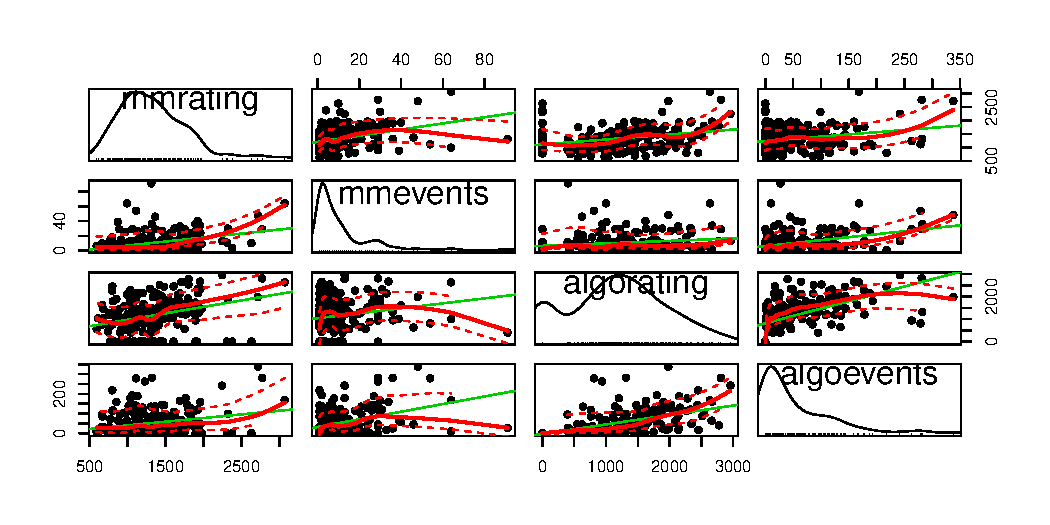
\includegraphics{Figures/unnamed-chunk-8-1.pdf}

Considerable geographic variation of registered participants.

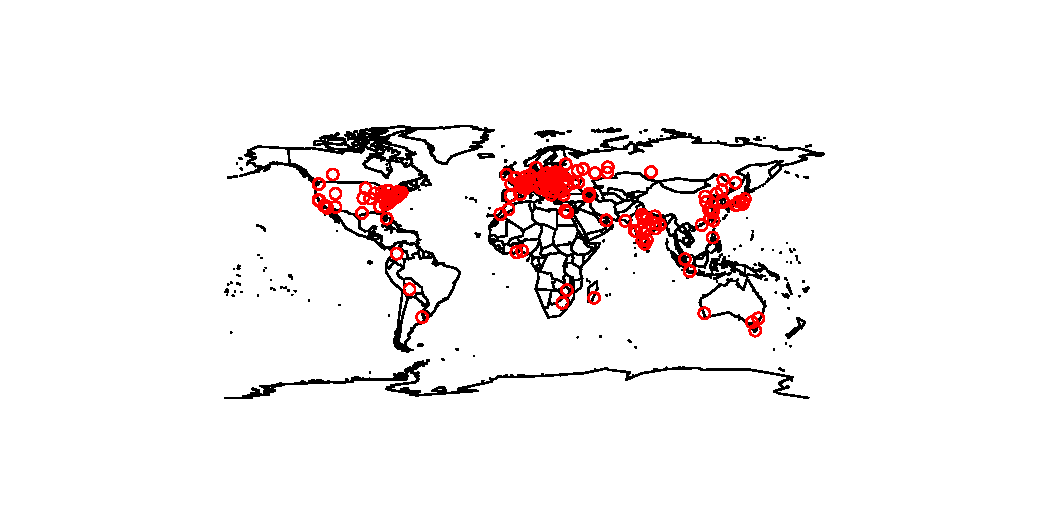
\includegraphics{Figures/unnamed-chunk-9-1.pdf}

\clearpage

\section{Results}\label{results}

In the eight-day submission period, we collected a total of 1759
submissions made by 86 participants. The frequency distribution of
submissions was rather skewed with participants in the 90th percentile
making 50 more submissions than those in the 10th percentile.

\begin{verbatim}
##        
##         Race Tournament Reserve
##   FALSE   73         67      73
##   TRUE    26         33      27
\end{verbatim}

Participation across treatments was higher in the Tournament treatment
(33 percent), followed by the Tournament w/reseve (27 percent), and the
Race treatment (26.263 percent). However, these differences are not
statistically significant (using a Fisher's Exact Test for Count Data
gives a p-value of 0.526)

\begin{figure}
\centering
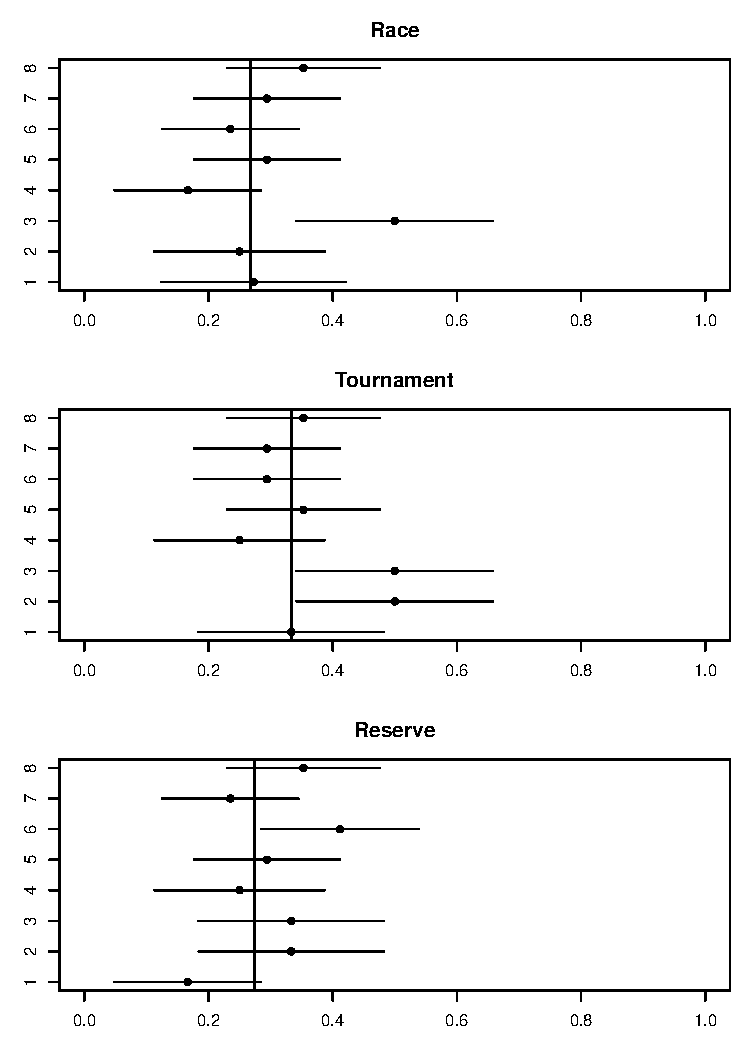
\includegraphics{Figures/unnamed-chunk-12-1.pdf}
\caption{Participation rates by rooms}
\end{figure}

Figure xxx shows the participation rates by rooms.

\begin{verbatim}
##        
##         Race Tournament Reserve
##   FALSE   84         81      85
##   TRUE    15         19      15
\end{verbatim}

Similar results are found when we consider only those who made
submissions above a score of xxxx. Participation across treatments was
higher in the Tournament treatment (19 percent), followed by the
Tournament w/reseve (15 percent), and the Race treatment (15.152
percent). However, these differences are not statistically significant
(using a Fisher's Exact Test for Count Data gives a p-value of 0.699)

\begin{verbatim}
##       Race Tournament    Reserve 
##         12          6         15
\end{verbatim}

Regarding to the frequency of submissions per participant, the median
count is larger in the race and in the tournament w/reserve (12 and 15
respectively) compared to the Tournament (a median of 6 submissions).
However, a Kruskal-Wallis rank sum test fails to reject the null
hypothesis (p=0.794) that at least one treatment was different in the
location of the frequency distribution of the submissions.

\begin{verbatim}
##       Race Tournament    Reserve 
##      0.799      0.805      0.808
\end{verbatim}

Concerning the distribution of the scores on the last submission, the
median final scores was higher in the Tournament w/reserve treatment
(0.808), followed by the Tournament (0.805), and the Race treatment
(0.799). As before, however, these differences are not statistically
significant (a Kruskal-Wallis rank sum test gives a p-value of 0.577).

Finally, let us focus on the timing of the first and last submission.
xxxx

\begin{figure}
\centering
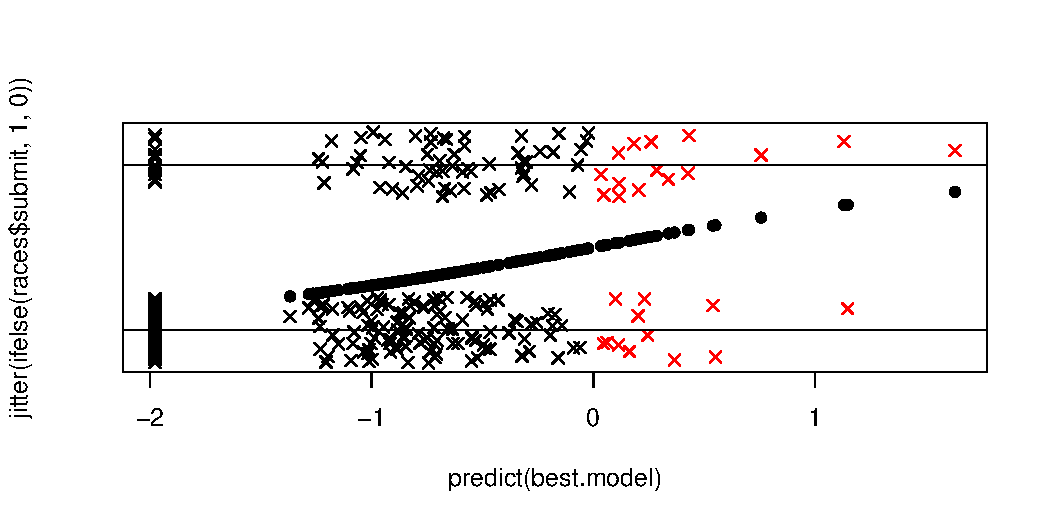
\includegraphics{Figures/unnamed-chunk-17-1.pdf}
\caption{Submissions timing within the submission period}
\end{figure}

Here we consider the hours of the day on the 24h. We normalize the 24h
on the unit interval (here I think we should take into account the
different timezoes.)

\begin{figure}
\centering
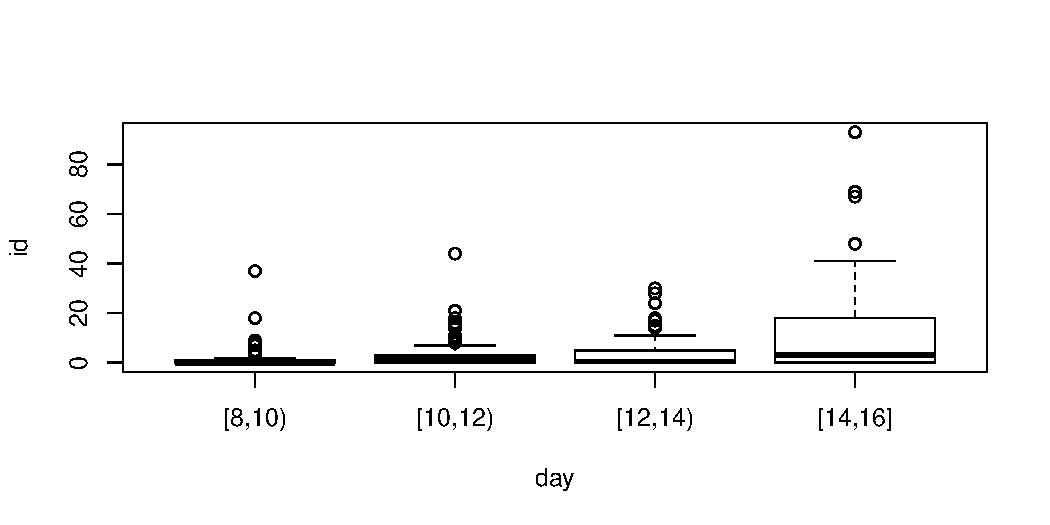
\includegraphics{Figures/unnamed-chunk-18-1.pdf}
\caption{Submissions within the 24h (need to adjust for timezone)}
\end{figure}

\subsection{Regressions}\label{regressions}

Although we do not find significant differences through an univariate
analysis, it is possible that differences will be xxx in a multivariate
analysis. Adding controls can indeed reduce noise and improve precisions
of our estimates.

Let's consider first a simple logistic model

\begin{verbatim}
## 
## Call:
## glm(formula = submit ~ treatment, family = quasibinomial, data = races)
## 
## Deviance Residuals: 
##    Min      1Q  Median      3Q     Max  
## -0.895  -0.793  -0.781   1.489   1.635  
## 
## Coefficients:
##                     Estimate Std. Error t value Pr(>|t|)
## (Intercept)          -1.0324     0.2295   -4.50  9.9e-06
## treatmentTournament   0.3242     0.3136    1.03     0.30
## treatmentReserve      0.0377     0.3224    0.12     0.91
## 
## (Dispersion parameter for quasibinomial family taken to be 1.01)
## 
##     Null deviance: 358.81  on 298  degrees of freedom
## Residual deviance: 357.49  on 296  degrees of freedom
## AIC: NA
## 
## Number of Fisher Scoring iterations: 4
\end{verbatim}

\begin{verbatim}
## 
## Call:
## glm(formula = submit ~ treatment + gender + educ + age + timezone + 
##     plang, family = quasibinomial, data = races)
## 
## Deviance Residuals: 
##    Min      1Q  Median      3Q     Max  
## -1.533  -0.840  -0.648   1.168   2.079  
## 
## Coefficients:
##                       Estimate Std. Error t value Pr(>|t|)
## (Intercept)            -1.8533     0.9969   -1.86    0.064
## treatmentTournament     0.2977     0.3381    0.88    0.379
## treatmentReserve        0.0454     0.3491    0.13    0.897
## genderMale              0.3312     0.6178    0.54    0.592
## educHigh School         0.8063     0.6322    1.28    0.203
## educMaster of Arts      0.2427     0.4906    0.49    0.621
## educBachelor            0.5050     0.5141    0.98    0.327
## age20-25 years old     -0.3094     0.6757   -0.46    0.647
## age26-30 years          0.5366     0.7060    0.76    0.448
## age31-40 years          0.9886     0.7021    1.41    0.160
## age41-50 years          0.4718     0.8314    0.57    0.571
## age51 years and above   1.1899     0.9109    1.31    0.193
## timezone                0.0109     0.0279    0.39    0.695
## plangC++               -0.1932     0.4441   -0.44    0.664
## plangJava              -0.8340     0.4754   -1.75    0.080
## plangOther             -0.4482     0.7454   -0.60    0.548
## plangPython             0.2196     0.5838    0.38    0.707
## plangVB                 1.1734     1.3532    0.87    0.387
## 
## (Dispersion parameter for quasibinomial family taken to be 1.06)
## 
##     Null deviance: 358.81  on 298  degrees of freedom
## Residual deviance: 337.25  on 281  degrees of freedom
## AIC: NA
## 
## Number of Fisher Scoring iterations: 4
\end{verbatim}

\begin{verbatim}
## 
## Call:
## glm(formula = submit ~ treatment + algorating + mmevents + algoevents + 
##     totalpayments, family = quasibinomial, data = races)
## 
## Deviance Residuals: 
##    Min      1Q  Median      3Q     Max  
## -1.713  -0.771  -0.644   1.040   1.908  
## 
## Coefficients:
##                            Estimate Std. Error t value Pr(>|t|)
## (Intercept)               -1.503410   0.327239   -4.59  6.5e-06
## treatmentTournament        0.372238   0.331949    1.12   0.2631
## treatmentReserve          -0.000123   0.343707    0.00   0.9997
## algorating                -0.000059   0.000228   -0.26   0.7957
## mmevents                   0.035712   0.013466    2.65   0.0084
## algoevents                 0.001907   0.003090    0.62   0.5377
## totalpayments1 - 599      -0.182154   0.477411   -0.38   0.7031
## totalpayments600 - 4500    0.226796   0.456516    0.50   0.6197
## totalpayments4500 - 37000  0.723311   0.426958    1.69   0.0913
## totalpayments>37000        0.466569   0.452361    1.03   0.3032
## 
## (Dispersion parameter for quasibinomial family taken to be 1.03)
## 
##     Null deviance: 358.81  on 298  degrees of freedom
## Residual deviance: 334.04  on 289  degrees of freedom
## AIC: NA
## 
## Number of Fisher Scoring iterations: 4
\end{verbatim}

\begin{verbatim}
## 
## Call:
## glm(formula = submit ~ treatment + algorating + mmevents + algoevents + 
##     totalpayments + gender + educ + age + timezone + plang, family = quasibinomial, 
##     data = races)
## 
## Deviance Residuals: 
##    Min      1Q  Median      3Q     Max  
## -1.966  -0.759  -0.597   0.992   2.211  
## 
## Coefficients:
##                            Estimate Std. Error t value Pr(>|t|)
## (Intercept)               -2.13e+00   1.07e+00   -1.99    0.047
## treatmentTournament        3.50e-01   3.56e-01    0.98    0.327
## treatmentReserve          -5.13e-03   3.70e-01   -0.01    0.989
## algorating                -3.52e-05   2.62e-04   -0.13    0.893
## mmevents                   3.50e-02   1.61e-02    2.17    0.031
## algoevents                 1.65e-03   3.34e-03    0.50    0.621
## totalpayments1 - 599      -2.12e-02   5.18e-01   -0.04    0.967
## totalpayments600 - 4500    2.56e-01   5.07e-01    0.50    0.614
## totalpayments4500 - 37000  7.25e-01   4.68e-01    1.55    0.123
## totalpayments>37000        3.60e-01   5.11e-01    0.70    0.482
## genderMale                 2.56e-01   6.51e-01    0.39    0.694
## educHigh School            8.29e-01   6.66e-01    1.24    0.215
## educMaster of Arts         1.39e-01   5.17e-01    0.27    0.788
## educBachelor               4.14e-01   5.43e-01    0.76    0.446
## age20-25 years old        -2.84e-01   7.17e-01   -0.40    0.692
## age26-30 years             3.45e-01   7.61e-01    0.45    0.651
## age31-40 years             6.57e-01   7.65e-01    0.86    0.391
## age41-50 years            -2.77e-01   9.49e-01   -0.29    0.770
## age51 years and above      5.57e-01   1.02e+00    0.55    0.584
## timezone                   1.17e-02   3.03e-02    0.39    0.700
## plangC++                  -4.17e-02   4.72e-01   -0.09    0.930
## plangJava                 -6.66e-01   4.99e-01   -1.34    0.183
## plangOther                -2.35e-03   7.83e-01    0.00    0.998
## plangPython                3.38e-01   6.13e-01    0.55    0.582
## plangVB                    7.60e-01   1.51e+00    0.50    0.615
## 
## (Dispersion parameter for quasibinomial family taken to be 1.09)
## 
##     Null deviance: 358.81  on 298  degrees of freedom
## Residual deviance: 320.83  on 274  degrees of freedom
## AIC: NA
## 
## Number of Fisher Scoring iterations: 4
\end{verbatim}

\begin{verbatim}
## 
## =====================================================
##                              Dependent variable:     
##                          ----------------------------
##                                     submit           
##                               (1)            (2)     
## -----------------------------------------------------
## poly(mmevents, deg = 3)1   12.200***                 
##                             (4.120)                  
##                                                      
## poly(mmevents, deg = 3)2     1.210                   
##                             (6.130)                  
##                                                      
## poly(mmevents, deg = 3)3     8.110*                  
##                             (4.740)                  
##                                                      
## poly(mmevents, deg = 2)1                   4.690*    
##                                            (2.540)   
##                                                      
## poly(mmevents, deg = 2)2                   -0.212    
##                                            (2.470)   
##                                                      
## poly(mmrating, deg = 2)1                  10.100***  
##                                            (3.120)   
##                                                      
## poly(mmrating, deg = 2)2                   -0.942    
##                                            (2.380)   
##                                                      
## Constant                   -0.961***      -1.020***  
##                             (0.138)        (0.143)   
##                                                      
## -----------------------------------------------------
## Observations                  299            299     
## Log Likelihood              -166.000      -164.000   
## Akaike Inf. Crit.           341.000        337.000   
## =====================================================
## Note:                     *p<0.1; **p<0.05; ***p<0.01
\end{verbatim}

\begin{verbatim}
## Analysis of Deviance Table
## 
## Model: binomial, link: logit
## 
## Response: submit
## 
## Terms added sequentially (first to last)
## 
## 
##                         Df Deviance Resid. Df Resid. Dev Pr(>Chi)
## NULL                                      298        359         
## poly(mmevents, deg = 2)  2     20.4       296        338  3.7e-05
## poly(mmrating, deg = 2)  2     11.1       294        327   0.0039
\end{verbatim}

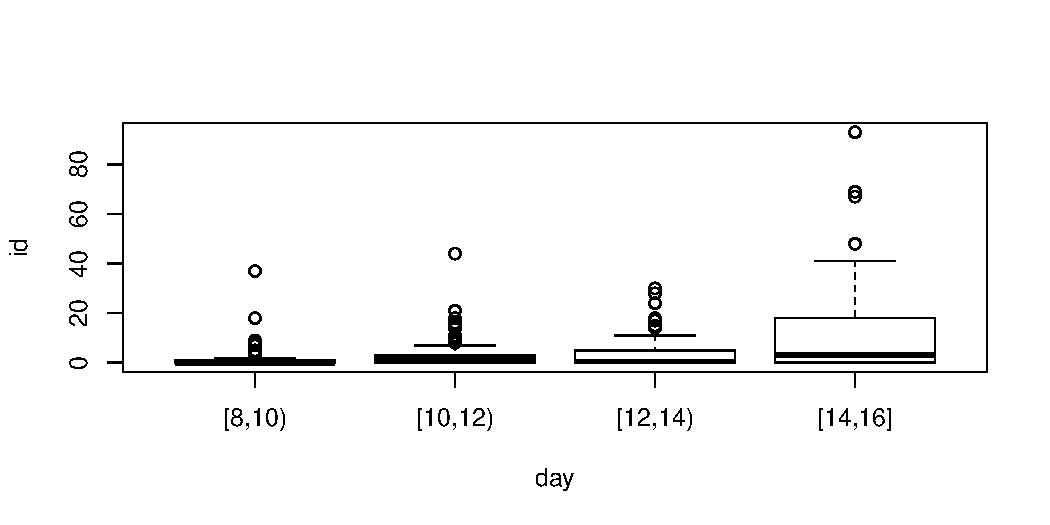
\includegraphics{Figures/unnamed-chunk-20-1.pdf}

This result does not seem to correlate well with the competitor's
experience or skills, as the Pearsons's correlation coefficient between
the count of past competitions or the rating and the count of
submissions is positive but generally low; see Table XXX. Thus,
differences in submissions appear idiosyncratic and perhaps related to
the way to organize the work rather than systematically associated with
underlying differences in experience or skills.

The timing of submissions was rather uniform during the submission
period with a peak of submissions made in the last of the competition.
(explain more)

\begin{verbatim}
#scores$submax <- ave(races.sub$id, races.sub$handle, FUN=max)
#par(mfrow=c(2, 1), mar=c(4,4,2,2))
#plot(subid==1 ~ as.POSIXct(subts), data=scores, type='h', yaxt='n'
#    , xlab='', ylab='', main='Dispersion time first submission')
#plot(subid==submax ~ as.POSIXct(subts), data=scores, type='h'
#    , yaxt='n', xlab='', ylab='', main='Dispersion time last submission')
\end{verbatim}

Proportions by rooms.

\begin{verbatim}
nsub <- tapply(races.sub$id, races.sub$handle, length)
races$submit <- races$handle %in% names(nsub)
treat <- tapply(races$treatment, races$room, unique)
n1 <- tapply(races$submit, races$room, sum)
n <- tapply(races$submit, races$room, length)
p <- (n1 + 1) / (n + 2)
SE <- sqrt(p*(1-p) / (n+2))
CI <- cbind(p+1.96*SE, p - 1.96*SE)

# All rooms
plot(p, 1:length(p), xlim=c(-0.1, 1), yaxt='n', bty='n', ann=FALSE, col=treat, pch=16)
segments(y0=1:length(p), x0=p+SE, x1=p-SE, col=treat, lwd=3)
segments(y0=1:length(p), x0=CI[, 1], x1=CI[, 2], col=treat)
text(y=1:length(p), x=p, levels(races$treatment)[treat], pos=3, cex=0.5, xpd=TRUE)
abline(v=mean(races$submit))

# Large rooms
treat <- treat[n<15]
p <- p[n<15]
n <- n[n<15] 
SE <- sqrt(p*(1-p) / (n+2))
CI <- cbind(p+1.96*SE, p - 1.96*SE)
plot(p, 1:length(p), xlim=c(-0.1, 1), yaxt='n', bty='n', ann=FALSE, col=treat, pch=16)
segments(y0=1:length(p), x0=p+SE, x1=p-SE, col=treat, lwd=3)
segments(y0=1:length(p), x0=CI[, 1], x1=CI[, 2], col=treat)
text(y=1:length(p), x=p, levels(races$treatment)[treat], pos=3, cex=0.5, xpd=TRUE)
abline(v=mean(races$submit))

\end{verbatim}

Consider panel data!

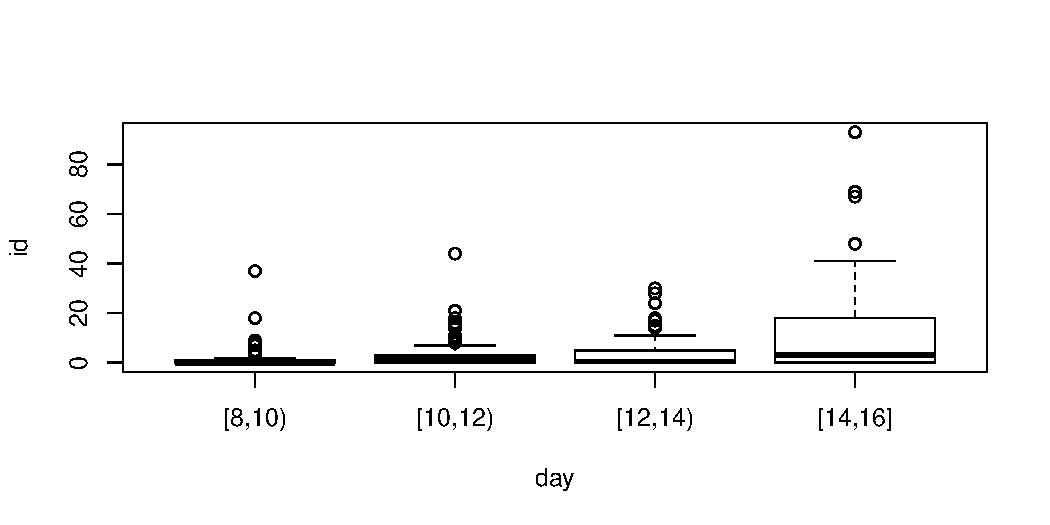
\includegraphics{Figures/unnamed-chunk-22-1.pdf}

\begin{verbatim}
## 
## Call:
## glm(formula = id ~ day, data = subs.long)
## 
## Deviance Residuals: 
##    Min      1Q  Median      3Q     Max  
## -11.69   -4.00   -1.59    0.08   81.31  
## 
## Coefficients:
##             Estimate Std. Error t value Pr(>|t|)
## (Intercept)     1.59       1.08    1.47     0.14
## day[10,12)      1.58       1.53    1.03     0.30
## day[12,14)      2.41       1.53    1.57     0.12
## day[14,16]     10.09       1.53    6.60  1.6e-10
## 
## (Dispersion parameter for gaussian family taken to be 101)
## 
##     Null deviance: 39401  on 343  degrees of freedom
## Residual deviance: 34190  on 340  degrees of freedom
## AIC: 2568
## 
## Number of Fisher Scoring iterations: 2
\end{verbatim}

\begin{verbatim}
## 
## Call:
## glm(formula = id ~ day, family = quasipoisson, data = subs.long)
## 
## Deviance Residuals: 
##    Min      1Q  Median      3Q     Max  
## -4.834  -2.828  -1.785   0.023  14.939  
## 
## Coefficients:
##             Estimate Std. Error t value Pr(>|t|)
## (Intercept)    0.466      0.342    1.36    0.174
## day[10,12)     0.689      0.419    1.65    0.101
## day[12,14)     0.921      0.404    2.28    0.023
## day[14,16]     1.993      0.365    5.47  8.9e-08
## 
## (Dispersion parameter for quasipoisson family taken to be 16)
## 
##     Null deviance: 4500.3  on 343  degrees of freedom
## Residual deviance: 3587.7  on 340  degrees of freedom
## AIC: NA
## 
## Number of Fisher Scoring iterations: 6
\end{verbatim}

\begin{verbatim}
## 
## Call:
## glm(formula = id > 0 ~ day, data = subs.long)
## 
## Deviance Residuals: 
##    Min      1Q  Median      3Q     Max  
## -0.733  -0.500   0.267   0.465   0.651  
## 
## Coefficients:
##             Estimate Std. Error t value Pr(>|t|)
## (Intercept)   0.3488     0.0521    6.70  8.7e-11
## day[10,12)    0.1860     0.0736    2.53    0.012
## day[12,14)    0.1512     0.0736    2.05    0.041
## day[14,16]    0.3837     0.0736    5.21  3.3e-07
## 
## (Dispersion parameter for gaussian family taken to be 0.233)
## 
##     Null deviance: 85.709  on 343  degrees of freedom
## Residual deviance: 79.279  on 340  degrees of freedom
## AIC: 481.4
## 
## Number of Fisher Scoring iterations: 2
\end{verbatim}

Scores: xxxx

\subsection{Treatment differences}\label{treatment-differences}

Difference in participation by treatments are show in Table XX.

\begin{verbatim}
Fisher's Exact Test for Count Data
\end{verbatim}

data: tab p-value = 0.5 alternative hypothesis: two.sided

We find no differences in the room size.

\begin{verbatim}
Fisher's Exact Test for Count Data
\end{verbatim}

data: tab p-value = 1 alternative hypothesis: true odds ratio is not
equal to 1 95 percent confidence interval: 0.569 1.691 sample estimates:
odds ratio 0.985

Ex-post

Timing: early vs late

Using a Chi-square test of independence, we find no significant
differences in participation rates associated with the assigned
treatments (p-value: 1); see Table XX.

Further, we model participation rates as a logistic regression. We use a
polynomial of third degree for the count of past competitions to account
for non-linear effects of experience; and we use an indicator for
whether the competitor had a win or not. Also, taking into account
differences in ability, participation rates are not significantly
different.

\subsection{Estimation results}\label{estimation-results}

Participation to the competition by treatment is shown in Figure
\ref{fig:entry}. Participation here is measured by the proportion of
registered participants per treatment who made any submission during the
eight-day submission period. Recall that competitors may decide to enter
into the competition and work on the problem without necessarily
submitting. In a tournament, for example, competitors are awarded a
prize based on their last submission and may decide to drop out without
submitting anything. However, this scenario seems unlikely. In fact,
competitors often end up making multiple submissions because by doing so
they obtain intermediate feedback via preliminary scoring (see Section
XXX for details). In a race, competitors have even stronger incentives
to make early submissions as any submission that hits the target first
wins.

\begin{verbatim}
Table xxx
\end{verbatim}

We find that the propensity to make a submission is higher in the
Tournament than in the Race and in the Tournament with reserve, but the
difference is not statistically significant (a Fisher's exact test gives
a p-value of xxxxx). As discussed in Section XXX, we may not have enough
power to detect differences below 5 percentage points. However, we find
the same not-significant result in a parametric regression analysis of
treatment differences with controls for the demographics and past
experience on the platform; see Table \ref{entry}. Adding individual
covariates reduces variability of outcomes, potentially increasing the
power of our test. In particular, Table \ref{entry} reports the results
from a logistic regression on the probability of making a submissions.
Column 1 reports the results from a baseline model with only treatment
dummies. Column 2 adds demographics controls, such as the age,
education, and gender. Column 3 adds controls for the past experience on
the platform. Across all these specifications, the impact of the
treatment dummies (including room size) on entry is not statistically
significant.

\subsection{Simulation results}\label{simulation-results}

\section{Empirical analysis}\label{empirical-analysis}

\subsection{Estimation results}\label{estimation-results-1}

Participation to the competition by treatment is shown in Figure
\[fig:entry\]. Participation here is measured by the proportion of
registered participants per treatment who made any submission during the
eight-day submission period. Recall that competitors may decide to enter
into the competition and work on the problem without necessarily
submitting. In a tournament, for example, competitors are awarded a
prize based on their last submission and may decide to drop out without
submitting anything. However, this scenario seems unlikely. In fact,
competitors often end up making multiple submissions because by doing so
they obtain intermediate feedback via preliminary scoring (see Section
XXX for details). In a race, competitors have even stronger incentives
to make early submissions as any submission that hits the target first
wins.

\begin{verbatim}
Table xxx
\end{verbatim}

We find that the propensity to make a submission is higher in the
Tournament than in the Race and in the Tournament with reserve, but the
difference is not statistically significant (a Fisher's exact test gives
a p-value of~xxxx). As discussed in Section XXX, we may not have enough
power to detect differences below 5 percentage points. However, we find
the same not-significant result in a parametric regression analysis of
treatment differences with controls for the demographics and past
experience on the platform; see Table \[entry\]. Adding individual
covariates reduces variability of outcomes, potentially increasing the
power of our test. In particular, Table \[entry\] reports the results
from a logistic regression on the probability of making a submissions.
Column 1 reports the results from a baseline model with only treatment
dummies. Column 2 adds demographics controls, such as the age,
education, and gender. Column 3 adds controls for the past experience on
the platform. Across all these specifications, the impact of the
treatment dummies (including room size) on entry is not statistically
significant.

\subsection{Simulation results}\label{simulation-results-1}

\renewcommand\refname{References}
\bibliography{/Users/andrea/Papers/library.bib}

\end{document}